\documentclass[11pt,a4paper]{report}
\usepackage[utf8]{inputenc}
\usepackage[english]{babel}
\usepackage[T1]{fontenc}
\usepackage{amsmath}
\usepackage{amsfonts}
\usepackage{amssymb}
\usepackage{makeidx}
\usepackage{graphicx}
\usepackage{float}
\usepackage{lmodern}
\usepackage[dvipsnames]{xcolor}
\usepackage{tikz}
\usetikzlibrary{intersections}
\usepackage{pgfplots}
\usetikzlibrary{calc}
\usepackage{geometry}
\geometry{hmargin=2cm,vmargin=2cm}
\usepackage{fancybox}
\usepackage{mathtools}
\usepackage{enumitem}
\usepackage{tcolorbox}
\usepackage{colortbl}
\usepackage{fancybox}
\tcbuselibrary{most}
\usepackage{pifont}
\usepackage[skip = 2pt, font = footnotesize]{caption}
\usepackage{subcaption}
\usepackage{eso-pic}
\usepackage{nicematrix}
\usepackage{multicol}
\usepackage{booktabs}
\usepackage{svg}
\usepackage{derivative}
\usepackage{wrapfig}
\usepackage{stmaryrd}
\usepackage{yfonts}
\usepackage[backend=biber]{biblatex}
\addbibresource{references.bib}
\author{Andrea}
\setlength{\columnsep}{.5cm}
\renewcommand{\thesection}{\Roman{section}}
\renewcommand{\thesubsection}{\arabic{subsection}}
\renewcommand{\thesubsubsection}{\alph{subsubsection}}
\usepackage{amsmath}
\colorlet{shadecolor}{cyan!15}
\usepackage{fancyhdr}
\usepackage{etoolbox}
\usepackage[export]{adjustbox}
\usepackage{fourier-orns}
\usepackage{lettrine}
\usepackage{physics}
\definecolor{RoyalRed}{RGB}{157,16, 45}
\usepackage{titlesec}
\usepackage{lipsum} 
\titleclass{\chapter}{straight}
\titleformat{\chapter}[display]
{\normalfont\bfseries\filcenter}
{\color{black}\LARGE\thechapter}
{1ex}
{\color{black}\titlerule[2pt]
\vspace{2ex}%
\LARGE}
[\vspace{1ex}%
{\titlerule[2pt]}]

\usepackage[export]{adjustbox}
\renewcommand{\headrule}{%
\vspace{6pt}\hrulefill
\raisebox{0pt}{\quad\decofourleft\decotwo\decofourright\quad}\hrulefill}
\pagestyle{fancy}
\fancyhf{}
\rhead{ \textcolor{black}{\footnotesize \today}}
\lhead{ENS}
\chead{ \textcolor{black}{· \emph{Turbulence characterization in tokamak} ·}}
\rfoot{Andrea Combette}
\fancyfoot[C]{\thepage} 

\newlength{\tabcont}

\setlength{\parindent}{0.0in}
\setlength{\parskip}{0.05in}

\setcounter{tocdepth}{4}
\setcounter{secnumdepth}{4}

\begin{document}
\begin{titlepage}
    \AddToShipoutPictureBG*{
        \begin{tikzpicture}[overlay,remember picture]
            \draw [line width=3pt]
            ($ (current page.north west) + (2cm,-2.0cm) $)
            rectangle
            ($ (current page.south east) + (-2cm,1.8cm) $);
            \draw [line width=1pt]
            ($ (current page.north west) + (2.15cm,-2.15cm) $)
            rectangle
            ($ (current page.south east) + (-2.15cm,1.95cm) $);
        \end{tikzpicture}
    }
    \begin{center}
        \vspace*{2cm}
        \emph{\footnotesize{Department of physics, École Normale Supérieure, Paris}}

        \emph{\footnotesize{Swiss Plasma Center, EPFL, Lausanne}}


        \vspace*{1cm}

        \textsc{Turbulence characterization}

        \textsc{In magnetically confined fusion research}
        \vspace*{1cm}

        \rule{14cm}{2pt}\vspace{.7cm}

        \Large{\textbf{Master Thesis 2024}}

        \vspace{.5cm}
        \rule{14cm}{2pt}
        \vspace{1cm}

        \Large Andrea Combette

        \vspace{3cm}

        \raisebox{-5pt}{\quad\decofourleft\decotwo\decofourright\quad}

        \vspace{2cm}
        \vspace{1cm}

        \begin{minipage}{14cm}
            \small{\textbf{Supervisors:}}
            \vspace{.5cm}

            \small{\textbf{Mr. Oleg Krutkin \null\hfill Pr. Jean François Allemand}}

        \end{minipage}
        \vspace{2cm}


        \begin{minipage}{14cm}
            \small{
                \textbf{Cautionary note : } This paper is a report on numerical methods for the shallow water equations and gravity waves. It is not intended to be a complete and rigorous study of the subject. The reader is invited to refer to the references for further details.
                It has been made by a Master Student, with some background in physics and mathematics, but no prior knowledge of the subject. It is therefore not intended to be a reference for experts in the field.}
        \end{minipage}

    \end{center}

\end{titlepage}

\newpage
\tableofcontents
\newpage


\begin{center}
    \vspace*{1.5cm}\Large{\textbf{Abstract}}
    \vspace*{1cm}
    \fontsize{11}{18}\selectfont

    \begin{minipage}{.7\linewidth}
        \lettrine[lines=4]{\color{black} O}{ne} of the common goals in experimental magnetically confined fusion research is characterization of the plasma turbulence. To that end, TCV tokamak features a novel short-pulse reflectometry (SPR) diagnostic, which can potentially be utilized to measure properties of the turbulence.
        It is essentially a radar system, where the plasma is probed by a short (under ns) microwave pulse in the presence of the cut-off (reflection) area from which the pulse reflects back into the probing antenna. The position of the cut-off for a particular probing frequency (in 50-75 GHz) range is determined by the plasma electron density. Thus, by measuring the delay between probing and reflected beam corresponding to different probing frequencies, the information about the electron density profile is inferred including its turbulent perturbations.
        Unfortunately, the complex interaction of microwaves with magnetized plasma makes it difficult to establish the connection between SPR measurements and properties of the turbulence. Numerical modeling utilizing the synthetic diagnostic approach was carried out to establish this connection for the case of low turbulence amplitudes (linear regime). However, the case of large turbulence amplitudes (nonlinear regime) is yet to be explored.
        Within the project a systematic analysis of the SPR diagnostic in the nonlinear regime will be carried out. The numerical finite difference code CUWA, which solves the wave equation for a given plasma density and provides synthetic reflected pulse will be utilized. The main goal of the project is identifying markers that can be used to determine if the diagnostic is operating in the nonlinear regime and assessing the possibility of determining the turbulence parameters regardless. Time permitting, the results of this analysis will be applied to the interpretation of experimental measurements and possibly used to develop a machine learning approach to analyzing SPR data.
    \end{minipage}
\end{center}

\newpage
\fontsize{10}{10}\selectfont
\begin{multicols}{2}
    \chapter{Theoretical Background}
    \section{Nuclear Fusion}
    \lettrine[lines=2, lhang=.3, nindent=0pt]{\color{black} T}{he} nuclear fusion reaction is the process by which two light atomic nuclei combine to form a heavier nucleus. It is accompanied by the release or absorption of energy depending on the masses of the nuclei involved. Indeed, the more the nuclei are light, the  more  energy is released due to the overcoming short-range nuclear force for light nuclei.
    However, to overcome the Coulomb barrier the reactant must be sufficiently close for a long enough time to allow the quantum tunnel effect between both particles. To do so, we must heat up the reactant to huge temperatures such that these latter are starting ionizing and turning into plasma.

    \subsection{Reaction}
    \begin{figure}[H]
        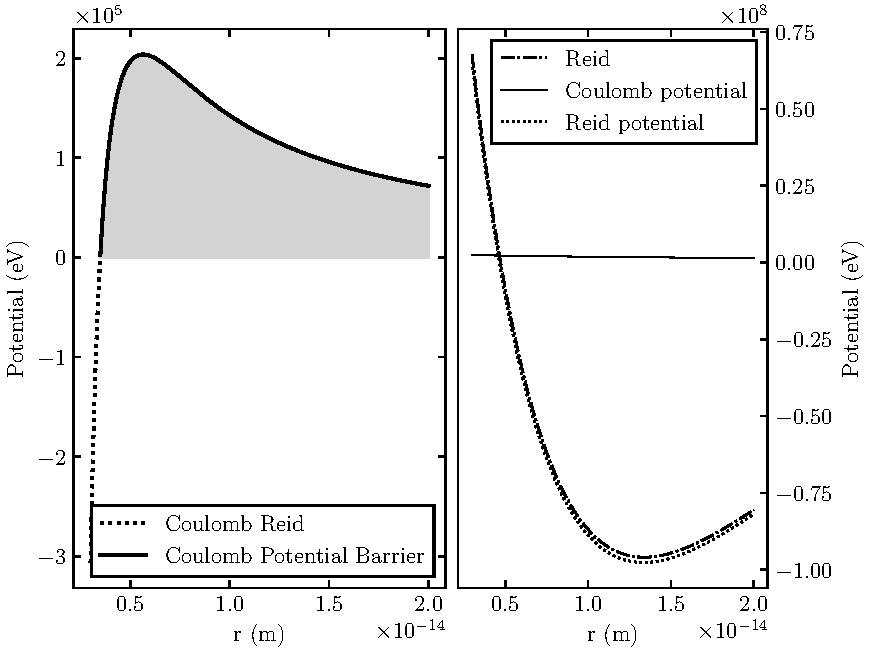
\includegraphics[width=1\linewidth]{./figures/potential_barrier2.pdf}
        \caption{Here we plot the residual Coulomb potential barrier between two proton considering the strong nuclear force as the Reid potential [cite]. On the right, the residual Reid potential.}
        \label{fig:barrier}
    \end{figure}
    Here it appears that the thermal energy needed to overcome the coulomb barrier is about : $$E_{\text{thermal}} \approx 0.2 \text{MeV}.$$This corresponds to a temperature of $2.5e^9$ K,  This is the reason why we need to heat up the plasma to such high temperatures. Note that the quick considerations are for proton-proton interaction, in fact the thermal energy needed is much smaller around $1e^8$ K for the deuterium-tritium reaction, due to quantum tunneling effect, and screening of coulomb potential by other nucleons:

    \subsubsection{D-T reaction}
    At the TCV the studied reaction is the deuterium-tritium reaction, which is the most promising reaction for fusion power, Indeed the energy barrier for the reaction to happen is about $70$ keV, whereas for deuterium-deuterium reaction it's $0.$1MeV,and for the deuterium-Helium it's about $0.2$MeV. The reaction is the following:
    \begin{align*}
        \text{D}^2 + \text{T}^3 & \rightarrow \text{He}^4 + \text{n(17.6 MeV)}
    \end{align*}
    The liberated energy is big enough to sustain the reaction, but it has a given probability to happen, and a positive energy yield is necessary to use the nuclear fusion reaction.
    A possible measure of this probability is the fusion cross-sectional area, which is much more that just a geometrical cross-section.
    \subsubsection{Fusion Cross-section}
    The fusion cross section is enhanced by the tunneling effect transparency ($T$) and by the reaction characteristics $R$. It is given by the following formula :
    $$\sigma \approx \sigma _{\text{geometry}}\times T\times R,$$

    where $\sigma _{\text{geometry}}$ is the geometrical cross-section, $T$ is the tunneling effect transparency, and $R$ is the reaction characteristics. The tunneling effect transparency is given by the Gamow factor, and the reaction characteristics given by the astrophysical S-factor.
    \subsubsection{Energy balance and Lawson criterion}
    $ \tau _{E}={\frac {W}{P_{\mathrm {loss} }}}$

    For the deuterium–tritium reaction, the physical value is at least

    $$n \tau E \ge 1.5.10^{20}{\frac {\mathrm {s} }{\mathrm {m} ^{3}}}$$
    Different regimes of confinement : Magnetic, Inertial, \dots
    \subsection{Tokamak}
    Magnetic confinement, plasma physics, \dots

    \section{{Plasma Turbulence}}
    \subsection{Characterization}
    instabilities grow due to inverse cascade of energy (2D geometry) --> scale
    \subsection{Diagnostics}
    \subsubsection{Doppler Reflectometry}
    Doppler reflectometry is a radar technique that measures the density fluctuations in a plasma. It is based on the interaction between probing microwave  and the turbulence, indeed the back-scattered wave by the plasma, is amplitude and phase dependent of many turbulence parameters. The Doppler shift is proportional to the velocity of the plasma fluctuations along the direction of the probing wave. The technique is used to measure the density fluctuations in the edge of the plasma, where the turbulence is strongest. The technique is also used to measure the radial electric field in the edge of the plasma, which is important for understanding the transport of particles and heat in the plasma. Doppler reflectometry is used in the TCV tokamak to measure the turbulence parameters (amplitude, mode number ... ).

    \subsubsection{RCDR}
    RCDR is a advanced Doppler Reflectometry technique it allows to measure the radial correlation length of the turbulences, using CCF. The principle is the following, we vary the probing wave frequency and we measure the correlation of the back-scattered wave. The correlation length is then deduced from the CCF function analysis.

    \subsubsection{Short Pulse Reflectometry}
    SPR is a radar technique that measures the density fluctuations in a plasma. It is based on the interaction between probing microwave  and the turbulence, indeed the back-scattered wave by the plasma, is amplitude and phase dependent of many turbulence parameters. The technique is used to measure the density fluctuations in the edge of the plasma, where the turbulence is strongest. The technique is also used to measure the radial electric field in the edge of the plasma, which is important for understanding the transport of particles and heat in the plasma. SPR is used in the TCV tokamak to measure the turbulence parameters (amplitude, mode number ... ).
    \chapter{Numerical Modeling}
    \section{Numerical Integration for plasma density}
    \section{Full wave Modelling}

    \begin{figure}[H]
        \centering
        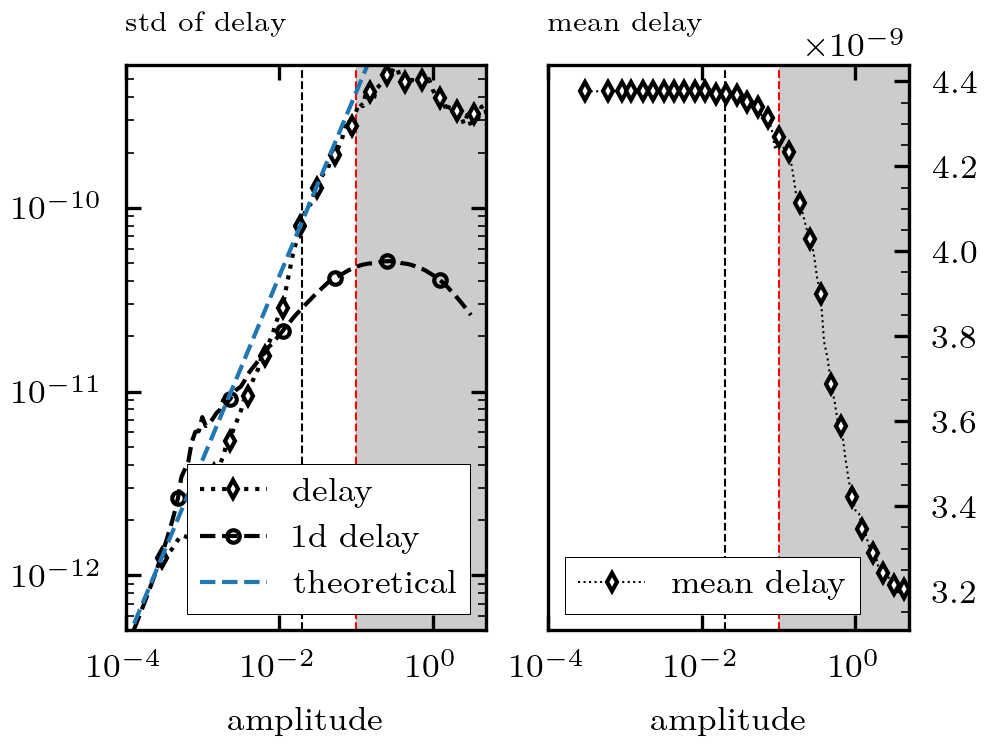
\includegraphics[width=1\linewidth]{./figures/delay_amp_4.png}
        \caption{Here we plot the residual Coulomb potential barrier between two proton considering the strong nuclear force as the Reid potential [cite]. On the right, the residual Reid potential.}
        \label{fig:barrier}
    \end{figure}

\end{multicols}
\printbibliography
\end{document}